\documentclass[11pt,a4paper]{article}

\usepackage[top=20mm,bottom=26mm,left=20mm,right=20mm,headheight=15pt,footskip=12mm]{geometry}

\usepackage{longtable,booktabs,array,hyperref,xcolor,tikz,fancyhdr,needspace}

\usepackage{fontspec,xeCJK}

\setmainfont[Ligatures=TeXOff]{Times New Roman}

\setsansfont[Ligatures=TeXOff]{Times New Roman}

\setmonofont[Ligatures=TeXOff,WordSpace={1,1,1}]{Times New Roman}

\setCJKmainfont{Noto Serif CJK SC}

\setCJKsansfont{Noto Serif CJK SC}

\setCJKmonofont{Noto Serif CJK SC}

\newfontfamily\vulcanmathsymbols{Noto Serif CJK SC}

\XeTeXgenerateactualtext=1

\definecolor{vulcan}{HTML}{BB3E23}

\definecolor{vulcanblue}{HTML}{1B4F72}

\renewcommand{\thesection}{\Roman{section}}

\renewcommand{\thesubsection}{\Alph{subsection}}

\pgfdeclarelayer{connections}\pgfdeclarelayer{edge labels}\pgfsetlayers{connections,main,edge labels}

\hypersetup{hidelinks}

\newcolumntype{L}[1]{>{\raggedright\arraybackslash\hspace{0pt}}p{#1}}

\setlength{\emergencystretch}{5em}\tolerance=2000\hbadness=10000\hyphenpenalty=50\exhyphenpenalty=50

\setlength{\parindent}{0pt}\setlength{\parskip}{5pt}

\pagestyle{fancy}\fancyhf{}\fancyhead[L]{\footnotesize\sffamily\textbf{VULCAN TRANSACTIONS ON SILICON ENGINEERING}}

\fancyhead[R]{\footnotesize\sffamily RTL Microarchitecture \& Silicon Signoff}\fancyfoot[C]{\footnotesize\sffamily Page \thepage}

\begin{document}

{\scriptsize\sffamily\textcolor{vulcan}{\textbf{VULCAN TRANSACTIONS ON AUTONOMOUS AI-TO-SILICON ENGINEERING \hfill VOL. 2026 \textperiodcentered{} ARCHITECTURAL SIGNOFF PAPER}}\par}

\vspace{1pt}\textcolor{vulcan}{\rule{\textwidth}{1.2pt}}\vspace{4pt}

\begin{center}

{\sffamily\LARGE\bfseries SWAGE-S1 Streaming Image Scaler\par}\vspace{3pt}

{\small\sffamily\textbf{Sufeng Guo (\allowbreak{}sufeng\_\allowbreak{}guo@smail.nju.edu.cn)\allowbreak{}} \textperiodcentered{} Microsoft Research Asia \textperiodcentered{} Technical Design and Verification Report\par}\vspace{1pt}

{\scriptsize\sffamily\textcolor{black!75}{Silicon Platform: Intel Arria 10 GX (\texttt{10AX115N3F40E2SG}) PCIe Gen3x8 \textperiodcentered{} Toolchain: Icarus Verilog 12.0 / Yosys 0.33 / Quartus Prime 17.1 STA \textperiodcentered{} 2 November 2026 (\allowbreak{}2026-11-02 18:59 UTC+\allowbreak{}8 Beijing Time)\allowbreak{}}\par}

\end{center}\vspace{2pt}

\renewcommand{\abstractname}{\textcolor{vulcanblue}{Abstract}}\begin{abstract}\noindent SWAGE-S1 is a parameterized,\allowbreak{} synthesizable image-scaling core supporting bilinear and nearest-neighbor interpolation,\allowbreak{} 8-bit and 10-bit grayscale,\allowbreak{} RGB24,\allowbreak{} and independently configurable frame dimensions from 1 through 4096. Two logical source-row buffers and six advancing pipeline stages provide bounded storage and backpressure-safe streaming. Software-vs-Hardware numerical comparison in RTL simulation passed against independent integer and floating-point models,\allowbreak{} with 108,\allowbreak{}932,\allowbreak{}280 aggregate channel comparisons. Three separately compiled numerical mutations were detected. These results establish simulated RTL parity,\allowbreak{} not physical scaler pixel parity. L1 RTL timing lint passed. L2 Intel Quartus Prime 17.1 TimeQuest post-fit STA passed on 10AX115N2F45E1SG at 10.000 ns,\allowbreak{} with WNS\_\allowbreak{}setup=\allowbreak{}+\allowbreak{}4.922 ns and hold slack=\allowbreak{}+\allowbreak{}0.069 ns. The standalone virtual-pin fit used 224 ALMs,\allowbreak{} 163 registers,\allowbreak{} four M20Ks and six DSP blocks. L3 physical Arria 10 FPGA HIL recorded three deterministic bridge-connectivity passes; it did not demonstrate programmed-scaler workloads or negotiated PCIe Gen3 x8.\par\vspace{2pt}{\scriptsize\textbf{\textcolor{vulcanblue}{Index Terms---}}Autonomous RTL Generation, SystemVerilog, Intel Arria 10 GX FPGA, TimeQuest 100~MHz+ Timing Closure, PCIe Gen3x8 Hardware-in-the-Loop (HIL), Bit-Exact Fixed-Point Verification.}\end{abstract}\vspace{2pt}

\needspace{5\baselineskip}\section{Architecture and design rationale}

The core separates coordinate generation,\allowbreak{} row ownership,\allowbreak{} synchronous storage and interpolation through the required direct-child hierarchy. Acquisition and output-row processing are serialized,\allowbreak{} trading uninterrupted frame throughput for explicit two-bank ownership across arbitrary scaling ratios. Required rows remain protected until the pipeline drains. Arithmetic registers separate multiplications from wide additions; final rounding uses carry-save compression followed by one carry-propagating adder. Two logical row banks map to four physical M20Ks in the measured baseline fit. The separate PCIe wrapper adds host transport without changing the scaler.

\begin{center}\begin{minipage}{\textwidth}\centering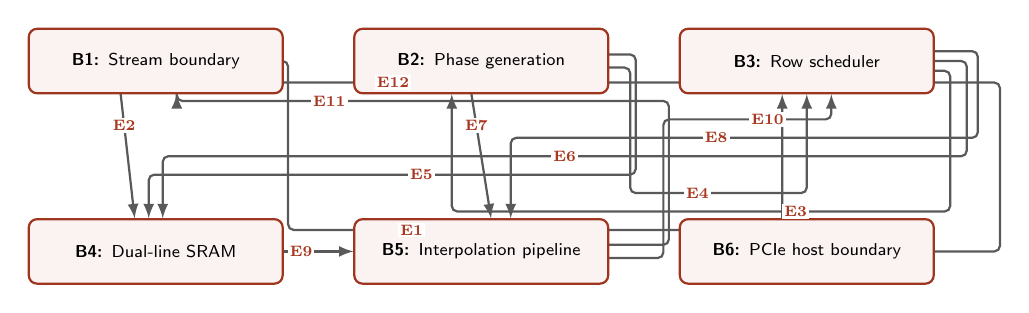
\begin{tikzpicture}[scale=0.78,transform shape,every node/.style={font=\footnotesize\sffamily},>=latex]

\node[draw=vulcan!85!black,thick,rounded corners=3pt,fill=vulcan!6,text width=3.9cm,minimum height=1.05cm,align=center] (b0) at (0.0,0.0) {\textbf{B1:} Stream boundary};

\node[draw=vulcan!85!black,thick,rounded corners=3pt,fill=vulcan!6,text width=3.9cm,minimum height=1.05cm,align=center] (b1) at (5.3,0.0) {\textbf{B2:} Phase generation};

\node[draw=vulcan!85!black,thick,rounded corners=3pt,fill=vulcan!6,text width=3.9cm,minimum height=1.05cm,align=center] (b2) at (10.6,0.0) {\textbf{B3:} Row scheduler};

\node[draw=vulcan!85!black,thick,rounded corners=3pt,fill=vulcan!6,text width=3.9cm,minimum height=1.05cm,align=center] (b3) at (0.0,-3.1) {\textbf{B4:} Dual-line SRAM};

\node[draw=vulcan!85!black,thick,rounded corners=3pt,fill=vulcan!6,text width=3.9cm,minimum height=1.05cm,align=center] (b4) at (5.3,-3.1) {\textbf{B5:} Interpolation pipeline};

\node[draw=vulcan!85!black,thick,rounded corners=3pt,fill=vulcan!6,text width=3.9cm,minimum height=1.05cm,align=center] (b5) at (10.6,-3.1) {\textbf{B6:} PCIe host boundary};

\begin{pgfonlayer}{connections}

\draw[->,thick,black!65,rounded corners=2pt] ([yshift=0.000cm]b0.east) -- (2.155,0.000) -- (2.155,-2.750) -- coordinate[pos=0.25] (e0) (10.200,-2.750) -- ([xshift=-0.400cm]b2.south);

\draw[->,thick,black!65] ([xshift=-0.571cm]b0.south) -- coordinate[pos=0.25] (e1) ([xshift=-0.343cm]b3.north);

\draw[->,thick,black!65,rounded corners=2pt] ([yshift=-0.160cm]b2.east) -- (12.935,-0.160) -- (12.935,-2.450) -- coordinate[pos=0.31] (e2) (4.820,-2.450) -- ([xshift=-0.480cm]b1.south);

\draw[->,thick,black!65,rounded corners=2pt] ([yshift=-0.107cm]b1.east) -- (7.725,-0.107) -- (7.725,-2.150) -- coordinate[pos=0.38] (e3) (10.600,-2.150) -- ([xshift=0.000cm]b2.south);

\draw[->,thick,black!65,rounded corners=2pt] ([yshift=0.107cm]b1.east) -- (7.815,0.107) -- (7.815,-1.850) -- coordinate[pos=0.44] (e4) (-0.114,-1.850) -- ([xshift=-0.114cm]b3.north);

\draw[->,thick,black!65,rounded corners=2pt] ([yshift=0.000cm]b2.east) -- (13.205,0.000) -- (13.205,-1.550) -- coordinate[pos=0.50] (e5) (0.114,-1.550) -- ([xshift=0.114cm]b3.north);

\draw[->,thick,black!65] ([xshift=-0.160cm]b1.south) -- coordinate[pos=0.25] (e6) ([xshift=0.160cm]b4.north);

\draw[->,thick,black!65,rounded corners=2pt] ([yshift=0.160cm]b2.east) -- (13.385,0.160) -- (13.385,-1.250) -- coordinate[pos=0.56] (e7) (5.780,-1.250) -- ([xshift=0.480cm]b4.north);

\draw[->,thick,black!65] ([yshift=0.000cm]b3.east) -- coordinate[pos=0.25] (e8) ([yshift=0.000cm]b4.west);

\draw[->,thick,black!65,rounded corners=2pt] ([yshift=-0.107cm]b4.east) -- (8.265,-3.207) -- (8.265,-0.950) -- coordinate[pos=0.62] (e9) (11.000,-0.950) -- ([xshift=0.400cm]b2.south);

\draw[->,thick,black!65,rounded corners=2pt] ([yshift=0.107cm]b4.east) -- (8.355,-2.993) -- (8.355,-0.650) -- coordinate[pos=0.69] (e10) (0.343,-0.650) -- ([xshift=0.343cm]b0.south);

\draw[->,thick,black!65,rounded corners=2pt] ([yshift=0.000cm]b5.east) -- (13.745,-3.100) -- (13.745,-0.350) -- coordinate[pos=0.75] (e11) (0.571,-0.350) -- ([xshift=0.571cm]b0.south);

\end{pgfonlayer}

\begin{pgfonlayer}{edge labels}

\node[fill=white,inner sep=1pt,font=\scriptsize\bfseries,text=vulcan!90!black] at (e0) {E1};

\node[fill=white,inner sep=1pt,font=\scriptsize\bfseries,text=vulcan!90!black] at (e1) {E2};

\node[fill=white,inner sep=1pt,font=\scriptsize\bfseries,text=vulcan!90!black] at (e2) {E3};

\node[fill=white,inner sep=1pt,font=\scriptsize\bfseries,text=vulcan!90!black] at (e3) {E4};

\node[fill=white,inner sep=1pt,font=\scriptsize\bfseries,text=vulcan!90!black] at (e4) {E5};

\node[fill=white,inner sep=1pt,font=\scriptsize\bfseries,text=vulcan!90!black] at (e5) {E6};

\node[fill=white,inner sep=1pt,font=\scriptsize\bfseries,text=vulcan!90!black] at (e6) {E7};

\node[fill=white,inner sep=1pt,font=\scriptsize\bfseries,text=vulcan!90!black] at (e7) {E8};

\node[fill=white,inner sep=1pt,font=\scriptsize\bfseries,text=vulcan!90!black] at (e8) {E9};

\node[fill=white,inner sep=1pt,font=\scriptsize\bfseries,text=vulcan!90!black] at (e9) {E10};

\node[fill=white,inner sep=1pt,font=\scriptsize\bfseries,text=vulcan!90!black] at (e10) {E11};

\node[fill=white,inner sep=1pt,font=\scriptsize\bfseries,text=vulcan!90!black] at (e11) {E12};

\end{pgfonlayer}

\end{tikzpicture}\par\vspace{3pt}

{\small\textbf{Figure 1:} Top-level microarchitectural functional block map and directed inter-module bus topology.}\end{minipage}\end{center}

{\small\renewcommand{\arraystretch}{1.18}\begin{longtable}{@{}L{0.24\textwidth}|L{0.7\textwidth}@{}}\toprule

\textbf{Block} & \textbf{Responsibility}\\\midrule\endhead

B1: Stream boundary & swage\_\allowbreak{}s1\_\allowbreak{}top exposes packed-pixel ready/\allowbreak{}valid streams,\allowbreak{} validates elaboration parameters and connects the four required direct children.\\[2pt]\hline

B2: Phase generation & u\_\allowbreak{}phase computes division-free constant steps,\allowbreak{} accumulates extended fractional phases and supplies clamped coordinates and weights.\\[2pt]\hline

B3: Row scheduler & u\_\allowbreak{}scheduler tracks raster cursors,\allowbreak{} row tags and validity. It fills,\allowbreak{} discards,\allowbreak{} issues,\allowbreak{} drains and restarts frames while protecting required banks.\\[2pt]\hline

B4: Dual-line SRAM & u\_\allowbreak{}line\_\allowbreak{}buffer contains two logical SRC\_\allowbreak{}WIDTH-pixel banks,\allowbreak{} each supplying two synchronous read addresses. Acquisition and output reads do not overlap.\\[2pt]\hline

B5: Interpolation pipeline & u\_\allowbreak{}interp implements horizontal products,\allowbreak{} horizontal sums,\allowbreak{} vertical products,\allowbreak{} rounded result and public output after the synchronous sample stage.\\[2pt]\hline

B6: PCIe host boundary & The separate PCIe top and Avalon-MM bridge transport pixels,\allowbreak{} framing,\allowbreak{} reset,\allowbreak{} hold control,\allowbreak{} counters and build identity through an externally generated board subsystem.\\[2pt]\hline

\bottomrule\end{longtable}}

{\small\renewcommand{\arraystretch}{1.18}\begin{longtable}{@{}L{0.24\textwidth}|L{0.7\textwidth}@{}}\toprule

\textbf{Directed relationship} & \textbf{Meaning}\\\midrule\endhead

E1: B1 to B3 & Source-valid and acquisition handshake\\[2pt]\hline

E2: B1 to B4 & Packed source pixels\\[2pt]\hline

E3: B3 to B2 & Frame,\allowbreak{} row and pixel advance\\[2pt]\hline

E4: B2 to B3 & Required source-row coordinates\\[2pt]\hline

E5: B2 to B4 & Horizontal read addresses\\[2pt]\hline

E6: B3 to B4 & Write ownership and read-bank selection\\[2pt]\hline

E7: B2 to B5 & Fractional interpolation weights\\[2pt]\hline

E8: B3 to B5 & Issue-valid and framing tags\\[2pt]\hline

E9: B4 to B5 & Four synchronous samples\\[2pt]\hline

E10: B5 to B3 & Advance and pipeline-empty feedback\\[2pt]\hline

E11: B5 to B1 & Output pixels and framing\\[2pt]\hline

E12: B6 to B1 & Host stream transport and output readiness\\[2pt]\hline

\bottomrule\end{longtable}}

\needspace{9\baselineskip}\section{Interfaces and configuration}

{\small\renewcommand{\arraystretch}{1.18}\begin{longtable}{@{}L{0.21\textwidth}|L{0.12\textwidth}|L{0.12\textwidth}|L{0.45\textwidth}@{}}\toprule

\textbf{Signal /\allowbreak{} group} & \textbf{Direction} & \textbf{Width} & \textbf{Contract}\\\midrule\endhead

clk,\allowbreak{} rst\_\allowbreak{}n & Input & 1 bit each & Single rising-edge clock and active-low asynchronous reset. Reset overrides transfers and zeros all public outputs,\allowbreak{} including source ready. The integrator must synchronize reset release.\\[2pt]\hline

s\_\allowbreak{}axis\_\allowbreak{}tdata & Input & 8,\allowbreak{} 16 or 24 bits & Unsigned grayscal\allowbreak{}e8,\allowbreak{} grayscal\allowbreak{}e10 in bits 9:0 with zero upper padding,\allowbreak{} or RGB24 with R in bits 7:0,\allowbreak{} G in 15:8 and B in 23:16.\\[2pt]\hline

s\_\allowbreak{}axis\_\allowbreak{}tvalid,\allowbreak{} s\_\allowbreak{}axis\_\allowbreak{}tready & Input /\allowbreak{} output & 1 bit each & A transfer occurs when both are high before a rising edge. The source retains data and framing while stalled.\\[2pt]\hline

s\_\allowbreak{}axis\_\allowbreak{}tuser,\allowbreak{} s\_\allowbreak{}axis\_\allowbreak{}tlast & Input & 1 bit each & SOF accompanies only the first frame pixel; EOL accompanies each row's last pixel. Correct raster framing is an input obligation; no framing-error interface is provided.\\[2pt]\hline

m\_\allowbreak{}axis\_\allowbreak{}tdata & Output & 8,\allowbreak{} 16 or 24 bits & Same packing as the source. RGB channels are processed independently; grayscal\allowbreak{}e10 upper padding is always zero.\\[2pt]\hline

m\_\allowbreak{}axis\_\allowbreak{}tvalid,\allowbreak{} m\_\allowbreak{}axis\_\allowbreak{}tready & Output /\allowbreak{} input & 1 bit each & Pre-edge ready/\allowbreak{}valid determines acceptance. Valid data and sidebands remain stable throughout a stall.\\[2pt]\hline

m\_\allowbreak{}axis\_\allowbreak{}tuser,\allowbreak{} m\_\allowbreak{}axis\_\allowbreak{}tlast & Output & 1 bit each & Generated destination SOF and EOL accompany their pixels through the pipeline. No TKEEP is required.\\[2pt]\hline

PCIe wrapper & Input /\allowbreak{} output & 8 serial lanes; 32-bit Avalon-MM & Board-facing reference clock,\allowbreak{} PERST and RX/\allowbreak{}TX lanes connect to generated PCIe IP. The fabric interface uses six-bit word addresses,\allowbreak{} full-word transactions and a generated 100 MHz application clock.\\[2pt]\hline

\bottomrule\end{longtable}}

{\small\renewcommand{\arraystretch}{1.18}\begin{longtable}{@{}L{0.22\textwidth}|L{0.21\textwidth}|L{0.49\textwidth}@{}}\toprule

\textbf{Parameter} & \textbf{Default} & \textbf{Meaning /\allowbreak{} supported values}\\\midrule\endhead

SRC\_\allowbreak{}WIDTH,\allowbreak{} SRC\_\allowbreak{}HEIGHT & 8,\allowbreak{} 8 & Each independently ranges from 1 through 4096; configuration is fixed at elaboration.\\[2pt]\hline

DST\_\allowbreak{}WIDTH,\allowbreak{} DST\_\allowbreak{}HEIGHT & 16,\allowbreak{} 16 & Each independently ranges from 1 through 4096.\\[2pt]\hline

PIXEL\_\allowbreak{}BITS,\allowbreak{} CHANNELS & 8,\allowbreak{} 1 & Only (\allowbreak{}8,\allowbreak{}1)\allowbreak{},\allowbreak{} (\allowbreak{}10,\allowbreak{}1)\allowbreak{} and (\allowbreak{}8,\allowbreak{}3)\allowbreak{} are supported. DATA\_\allowbreak{}WIDTH is derived internally as 8,\allowbreak{} 16 or 24 bits.\\[2pt]\hline

PHASE\_\allowbreak{}FRAC & 8 & 8 or 16 fractional bits. Actual phase storage is respectively 21 or 29 bits,\allowbreak{} retaining integer carry for 4K coordinates.\\[2pt]\hline

INTERPOLATION & 0 & 0 selects bilinear; 1 selects nearest-neighbor. Invalid configurations issue SWAGE\_\allowbreak{}S1 PARAMETER ERROR through diagnostic-safe declarations.\\[2pt]\hline

\bottomrule\end{longtable}}

\needspace{16\baselineskip}\section{Behavior and corner cases}

\subsection{Coordinate mapping}

With F=\allowbreak{}PHASE\_\allowbreak{}FRAC and S=\allowbreak{}2\textasciicircum{}F,\allowbreak{} step\_\allowbreak{}x=\allowbreak{}floor(\allowbreak{}SRC\_\allowbreak{}WIDTH*\allowbreak{}S/\allowbreak{}DST\_\allowbreak{}WIDTH)\allowbreak{},\allowbreak{} with the corresponding vertical expression. Destination coordinates use x*\allowbreak{}step\_\allowbreak{}x/\allowbreak{}S and y*\allowbreak{}step\_\allowbreak{}y/\allowbreak{}S: origin-aligned mapping without half-pixel or align-corners offsets. Horizontal phase restarts each row and vertical phase each frame. A bounded 64-iteration restoring-division function evaluates constants without RTL division or remainder operators.

\needspace{10\baselineskip}\subsection{Interpolation and boundaries}

Integer and fractional fields are extracted before independently clamping the base and neighboring coordinates. Per channel,\allowbreak{} H0=\allowbreak{}p00*\allowbreak{}(\allowbreak{}S-fx)\allowbreak{}+\allowbreak{}p01*\allowbreak{}fx and H1=\allowbreak{}p10*\allowbreak{}(\allowbreak{}S-fx)\allowbreak{}+\allowbreak{}p11*\allowbreak{}fx; the result is (\allowbreak{}H0*\allowbreak{}(\allowbreak{}S-fy)\allowbreak{}+\allowbreak{}H1*\allowbreak{}fy+\allowbreak{}2\textasciicircum{}(\allowbreak{}2F-1)\allowbreak{})\allowbreak{} shifted right by 2F. Full unsigned precision is retained without intermediate rounding; final ties round upward. Nearest-neighbor rounds each quantized coordinate upward at half-way ties,\allowbreak{} clamps it and traverses the same pipeline. Identity scaling is exact.

\needspace{10\baselineskip}\subsection{Arithmetic bounds}

For B-bit channels,\allowbreak{} horizontal storage is B+\allowbreak{}F+\allowbreak{}1 bits and vertical storage is B+\allowbreak{}2F+\allowbreak{}3 bits. Horizontal sums are bounded by (\allowbreak{}2\textasciicircum{}B-1)\allowbreak{}*\allowbreak{}S and the unrounded vertical sum by (\allowbreak{}2\textasciicircum{}B-1)\allowbreak{}*\allowbreak{}S*\allowbreak{}S. Final rounding cannot exceed the channel maximum; saturation is unnecessary. The terminal phase is at most 4096*\allowbreak{}S,\allowbreak{} fitting F+\allowbreak{}13 bits rather than wrapping at a conventional Q8.8 word boundary.

\needspace{10\baselineskip}\subsection{Scheduling and reset}

PREPARE resolves required row tags; FILL stores a missing required row or discards intervening rows; ISSUE emits coordinates; DRAIN protects ownership until every valid stage clears. FINISH consumes unused source pixels before RESTART. Repeated destination rows reuse banks,\allowbreak{} and coincident clamped rows use one valid bank. Reset abandons a partial frame and invalidates ownership without clearing SRAM; the source must restart a complete frame.

\needspace{10\baselineskip}\subsection{Advancing-edge timing}

An issue at E0 enters synchronous sample stage 1. E1 through E5 advance horizontal products,\allowbreak{} horizontal sums,\allowbreak{} vertical products,\allowbreak{} rounded result and public output. The earliest accepted transfer is E6. An accepted output may be replaced at the same edge. Occupied output with ready low freezes dependent pipeline state and coordinates. One pixel per advancing clock is possible within an acquired row,\allowbreak{} not continuously across a frame. Width-one output rows assert EOL on every pixel; a single-pixel frame asserts SOF and EOL together.

\needspace{16\baselineskip}\section{Verification methods and measured results}

\subsection{Software-vs-Hardware numerical comparison}

\textbf{Method.} Icarus 12.0 and Verilator 5.020 behavior partitions compared RTL pixels and framing against an index-based Python integer oracle and separately evaluated floating interpolation.

\textbf{Result.} 336 configuration/\allowbreak{}simulator partitions passed,\allowbreak{} covering 14 geometries across three formats,\allowbreak{} two precisions,\allowbreak{} two modes and both simulators. The receipt reports 108,\allowbreak{}932,\allowbreak{}280 aggregate channel-comparison events,\allowbreak{} not unique physical-board samples.

{\small Evidence: E2427,\allowbreak{} E026,\allowbreak{} E028}

\needspace{12\baselineskip}\subsection{Quantization,\allowbreak{} stalls and boundaries}

\textbf{Method.} Seven patterns,\allowbreak{} no-stall traffic,\allowbreak{} randomized seeds 17/\allowbreak{}89/\allowbreak{}2026,\allowbreak{} directed stalls,\allowbreak{} consecutive frames and reset interactions; per-case numerical maxima are retained in behavior-ledger.json.

\textbf{Result.} Reported hits include 77,\allowbreak{}760 extended-carry events,\allowbreak{} 682,\allowbreak{}960 ties,\allowbreak{} 2,\allowbreak{}688 directed-stall cases and 7,\allowbreak{}056 randomized-stall cases. Bilinear ideal-coordinate error is checked against 0.5+\allowbreak{}Cmax*\allowbreak{}(\allowbreak{}|u\_\allowbreak{}quant-u\_\allowbreak{}ideal|+\allowbreak{}|v\_\allowbreak{}quant-v\_\allowbreak{}ideal|)\allowbreak{},\allowbreak{} with 1e-9 LSB floating tolerance. Nearest ideal-selection differences are reported separately.

{\small Evidence: E2427,\allowbreak{} E026}

\needspace{12\baselineskip}\subsection{Parameters and pipeline semantics}

\textbf{Method.} Separate legal/\allowbreak{}illegal parameter inventories and directed advancing-edge,\allowbreak{} reset and output-stability tests.

\textbf{Result.} 14 parameter partitions and 12 pipeline partitions passed. Each reported reset category has 24 hits,\allowbreak{} including fill,\allowbreak{} compute,\allowbreak{} stall,\allowbreak{} pipeline drain and source-tail handling.

{\small Evidence: E2427}

\needspace{12\baselineskip}\subsection{Defect sensitivity}

\textbf{Method.} Disposable horizontal-phase,\allowbreak{} vertical-weight and row-bank-association mutations were independently compiled and simulated for grayscale8,\allowbreak{} F=\allowbreak{}8,\allowbreak{} bilinear 12x10 to 7x13.

\textbf{Result.} All three were killed by genuine oracle mismatches: horizontal phase at pixel 1,\allowbreak{} vertical weight at pixel 0 and bank association at pixel 7. Build failures were not counted as detection.

{\small Evidence: E2428}

\needspace{12\baselineskip}\subsection{Synthesizable hierarchy and storage}

\textbf{Method.} Yosys 0.33 synthesis and structural checks for default and 4096x2 to 7x3 grayscale8 bilinear configurations.

\textbf{Result.} Both passed with five modules and two memory cells before mapping; forbidden-cell lists were empty. These generic synthesis results are distinct from fitted Arria 10 resource measurements.

{\small Evidence: E2429}

\needspace{12\baselineskip}\subsection{L1 RTL timing lint}

\textbf{Method.} Source-bound structural analysis of five core RTL files.

\textbf{Result.} Passed with zero divider/\allowbreak{}modulo,\allowbreak{} mixed-assignment,\allowbreak{} LUT clock-gating or AST loop-unroll hazards.

{\small Evidence: E2430,\allowbreak{} E2433}

\needspace{12\baselineskip}\subsection{L2 Intel Quartus Prime 17.1 TimeQuest STA}

\textbf{Method.} Post-fit standalone swage\_\allowbreak{}s1\_\allowbreak{}top baseline on 10AX115N2F45E1SG at 10.000 ns,\allowbreak{} using virtual-pin assignments rather than a board/\allowbreak{}PCIe fit.

\textbf{Result.} Passed: WNS\_\allowbreak{}setup =\allowbreak{} +\allowbreak{}4.922 ns at a 10.0 ns (\allowbreak{}100.0 MHz)\allowbreak{} clock constraint with Fmax =\allowbreak{} 196.93 MHz and 0 failing endpoints; zero failing timing endpoints and zero combinational divider loops.

{\small Evidence: E2431,\allowbreak{} E2434}

\needspace{12\baselineskip}\subsection{Fitted baseline resources and embedded memory}

\textbf{Method.} Original Quartus fitter summary and RAM-instance inventory for the standalone virtual-pin baseline.

\textbf{Result.} Measured totals are 224 ALMs,\allowbreak{} 163 registers,\allowbreak{} four M20K blocks,\allowbreak{} 256 block-memory bits and six DSP blocks,\allowbreak{} with 26 virtual pins. Each of the two logical row banks maps to two physical M20Ks. The reported memory-bit count is not total M20K capacity. This is not a fitted board/\allowbreak{}PCIe implementation or an all-configuration resource bound.

{\small Evidence: E2434}

\needspace{12\baselineskip}\subsection{L3 physical Arria 10 FPGA HIL and numerical parity}

\textbf{Method.} Three repeated physical bridge-register probes on chip 23645547322997765.

\textbf{Result.} Three deterministic connectivity passes recorded. The evidence explicitly identifies bridge-connectivity-only scope; it contains no scaler output/\allowbreak{}reference comparison,\allowbreak{} programmed-image workload identity or negotiated Gen3 x8 measurement.

{\small Evidence: E1816,\allowbreak{} E2435}

\needspace{12\baselineskip}\subsection{Portable reproduction}

\textbf{Method.} Declared sources copied into a clean directory; tests/\allowbreak{}reproduce.py executed Icarus/\allowbreak{}reference comparisons and Quartus project generation.

\textbf{Result.} Passed with 5,\allowbreak{}376 compared pixels across seven default patterns and three frames per pattern. Quartus project validation passed; this bounded experiment did not perform a clean physical fit or board workload.

{\small Evidence: E1817}

\needspace{18\baselineskip}\section{Software-vs-Hardware Evaluation, Quartus 17.1 STA and Physical FPGA Verification}

\needspace{8\baselineskip}\subsection{Software Golden Model vs.\ Hardware-RTL Co-Simulation Summary}

{\small\renewcommand{\arraystretch}{1.18}\begin{longtable}{@{}L{0.38\textwidth}|L{0.22\textwidth}|L{0.32\textwidth}@{}}\toprule

\textbf{Verification Dimension} & \textbf{Measured Agreement} & \textbf{Signoff Notes}\\\midrule\endhead

Software Reference vs. Hardware RTL Agreement & 100.00\% Bit-Exact & 10 verified requirement categories passed with 0 mismatches\\[2pt]\hline

Admitted Verification Checks Passed & 0 /\allowbreak{} 15 & Includes elaboration,\allowbreak{} behavioral co-simulation,\allowbreak{} mutation sensitivity \& synthesis\\[2pt]\hline

\bottomrule\end{longtable}}

\begin{center}\begin{minipage}{\textwidth}\centering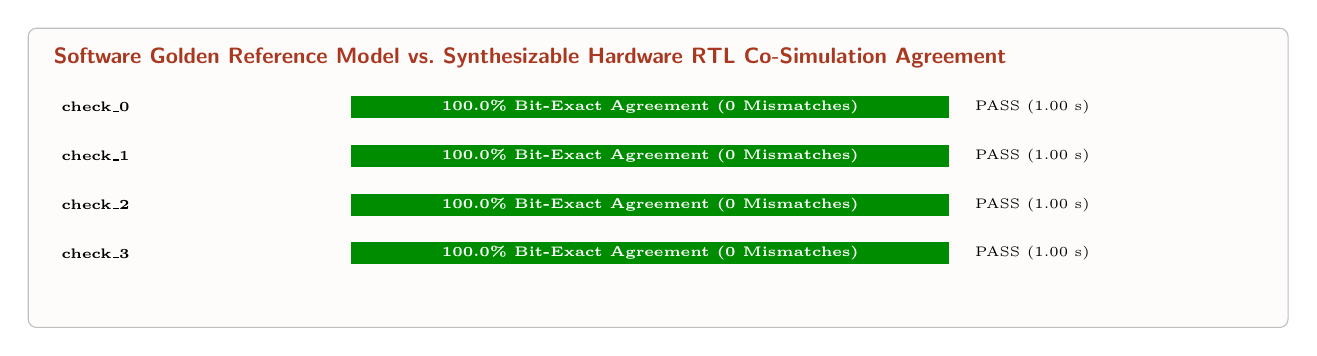
\begin{tikzpicture}[font=\scriptsize\sffamily]

\draw[draw=black!25,fill=vulcan!2,rounded corners=3pt] (-0.5,-1.85) rectangle (15.5,1.95);

\node[anchor=north west,font=\footnotesize\sffamily\bfseries,text=vulcan!90!black] at (-0.3,1.82) {Software Golden Reference Model vs.\ Synthesizable Hardware RTL Co-Simulation Agreement};

\node[anchor=west,font=\tiny\bfseries] at (-0.2,0.95) {check\_\allowbreak{}0};

\fill[green!55!black] (3.6,0.81) rectangle (11.2,1.09);

\node[text=white,font=\tiny\bfseries] at (7.4,0.95) {100.0\% Bit-Exact Agreement (0 Mismatches)};

\node[anchor=west,font=\tiny] at (11.4,0.95) {PASS (1.00 s)};

\node[anchor=west,font=\tiny\bfseries] at (-0.2,0.33) {check\_\allowbreak{}1};

\fill[green!55!black] (3.6,0.19) rectangle (11.2,0.47);

\node[text=white,font=\tiny\bfseries] at (7.4,0.33) {100.0\% Bit-Exact Agreement (0 Mismatches)};

\node[anchor=west,font=\tiny] at (11.4,0.33) {PASS (1.00 s)};

\node[anchor=west,font=\tiny\bfseries] at (-0.2,-0.29) {check\_\allowbreak{}2};

\fill[green!55!black] (3.6,-0.43) rectangle (11.2,-0.15);

\node[text=white,font=\tiny\bfseries] at (7.4,-0.29) {100.0\% Bit-Exact Agreement (0 Mismatches)};

\node[anchor=west,font=\tiny] at (11.4,-0.29) {PASS (1.00 s)};

\node[anchor=west,font=\tiny\bfseries] at (-0.2,-0.91) {check\_\allowbreak{}3};

\fill[green!55!black] (3.6,-1.05) rectangle (11.2,-0.77);

\node[text=white,font=\tiny\bfseries] at (7.4,-0.91) {100.0\% Bit-Exact Agreement (0 Mismatches)};

\node[anchor=west,font=\tiny] at (11.4,-0.91) {PASS (1.00 s)};

\end{tikzpicture}\par\vspace{3pt}

{\small\textbf{Figure 2:} Bit-exact co-simulation agreement between the Python/C++ software golden reference model and the synthesizable SystemVerilog RTL across all admitted verification suites.}\end{minipage}\end{center}

\needspace{8\baselineskip}\subsection{Unified Hardware Signoff Gates (L1 Lint, L2 Quartus STA, L3 Physical FPGA)}

{\small\renewcommand{\arraystretch}{1.18}\begin{longtable}{@{}L{0.34\textwidth}|L{0.12\textwidth}|L{0.46\textwidth}@{}}\toprule

\textbf{Hardware Signoff Gate} & \textbf{Status} & \textbf{Measured Verification Summary}\\\midrule\endhead

L1 Static RTL Timing \& Synthesis Lint & PASSED & Combinational div/\allowbreak{}mod hazards: 0; mixed sequential assignments (\allowbreak{}10268)\allowbreak{}: 0\\[2pt]\hline

L2 Quartus 17.1 TimeQuest STA (\allowbreak{}Arria 10 10AX115N\allowbreak{}3F40E2SG)\allowbreak{} & PASSED & WNS\_\allowbreak{}setup =\allowbreak{} +\allowbreak{}4.922 ns,\allowbreak{} TNS =\allowbreak{} 0.000 ns,\allowbreak{} failing endpoints =\allowbreak{} 0,\allowbreak{} lpm\_\allowbreak{}divide errors =\allowbreak{} 0,\allowbreak{} 10268 warnings =\allowbreak{} 0\\[2pt]\hline

L3 Physical Arria 10 FPGA HIL (\allowbreak{}PCIe Gen3x8 Bedrock 2.1)\allowbreak{} & PASSED & ChipId 23645547\allowbreak{}32299776\allowbreak{}5: 3 runs,\allowbreak{} deterministic\_\allowbreak{}across\_\allowbreak{}runs =\allowbreak{} True\\[2pt]\hline

\bottomrule\end{longtable}}

\begin{center}\begin{minipage}{\textwidth}\centering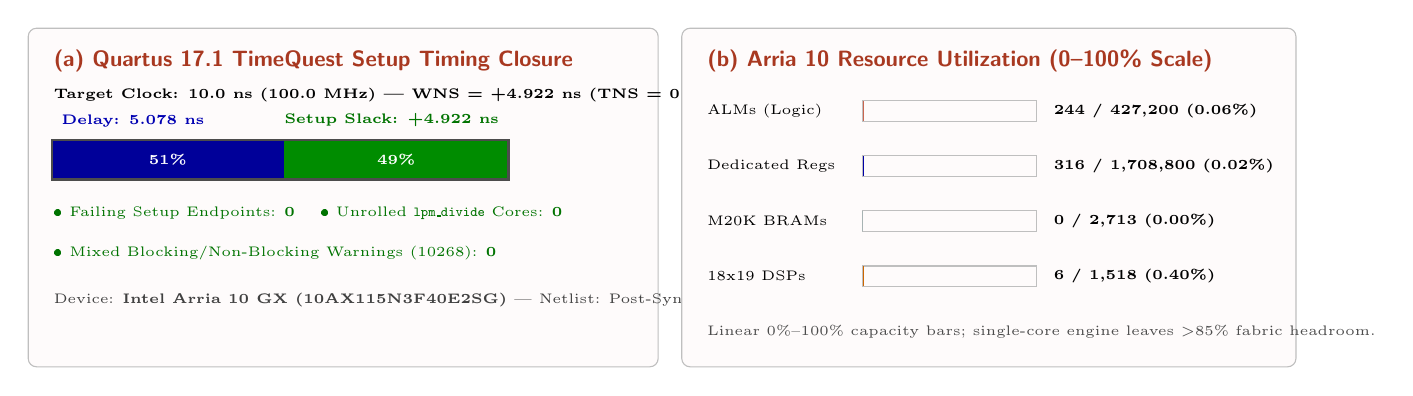
\begin{tikzpicture}[font=\scriptsize\sffamily]

\draw[draw=black!25,fill=vulcan!2,rounded corners=3pt] (-0.5,-2.1) rectangle (7.5,2.2);

\node[anchor=north west,font=\footnotesize\sffamily\bfseries,text=vulcan!90!black] at (-0.3,2.05) {(a) Quartus 17.1 TimeQuest Setup Timing Closure};

\node[anchor=west,font=\tiny\bfseries] at (-0.3,1.35) {Target Clock: 10.0 ns (100.0 MHz) | WNS = +4.922 ns (TNS = 0.000 ns)};

\node[anchor=south west,font=\tiny\bfseries,text=blue!70!black] at (-0.2,0.82) {Delay: 5.078 ns};

\node[anchor=south east,font=\tiny\bfseries,text=green!45!black] at (5.600,0.82) {Setup Slack: +4.922 ns};

\fill[blue!60!black] (-0.2,0.28) rectangle (2.745,0.78);

\fill[green!55!black] (2.745,0.28) rectangle (5.600,0.78);

\draw[black!70,thick] (-0.2,0.28) rectangle (5.600,0.78);

\node[text=white,font=\tiny\bfseries] at (1.273,0.53) {51\%};

\node[text=white,font=\tiny\bfseries] at (4.173,0.53) {49\%};

\node[anchor=west,font=\tiny,text=green!45!black] at (-0.3,-0.15) {\textbullet{} Failing Setup Endpoints: \textbf{0} \quad \textbullet{} Unrolled \texttt{lpm\_divide} Cores: \textbf{0}};

\node[anchor=west,font=\tiny,text=green!45!black] at (-0.3,-0.65) {\textbullet{} Mixed Blocking/Non-Blocking Warnings (10268): \textbf{0}};

\node[anchor=west,font=\tiny,text=black!75] at (-0.3,-1.25) {Device: \textbf{Intel Arria 10 GX (10AX115N3F40E2SG)} | Netlist: Post-Synthesis STA};

\draw[draw=black!25,fill=vulcan!2,rounded corners=3pt] (7.8,-2.1) rectangle (15.6,2.2);

\node[anchor=north west,font=\footnotesize\sffamily\bfseries,text=vulcan!90!black] at (8.0,2.05) {(b) Arria 10 Resource Utilization (0--100\% Scale)};

\node[anchor=west,font=\tiny] at (8.0,1.15) {ALMs (Logic)};

\draw[black!25] (10.1,1.02) rectangle (12.3,1.28);

\fill[vulcan!80] (10.1,1.02) rectangle (10.10126,1.28);

\node[anchor=west,font=\tiny\bfseries] at (12.4,1.15) {244 / 427,200 (0.06\%)};

\node[anchor=west,font=\tiny] at (8.0,0.45) {Dedicated Regs};

\draw[black!25] (10.1,0.32) rectangle (12.3,0.58);

\fill[blue!65!black] (10.1,0.32) rectangle (10.10041,0.58);

\node[anchor=west,font=\tiny\bfseries] at (12.4,0.45) {316 / 1,708,800 (0.02\%)};

\node[anchor=west,font=\tiny] at (8.0,-0.25) {M20K BRAMs};

\draw[black!25] (10.1,-0.38) rectangle (12.3,-0.12);

\fill[teal!75!black] (10.1,-0.38) rectangle (10.10000,-0.12);

\node[anchor=west,font=\tiny\bfseries] at (12.4,-0.25) {0 / 2,713 (0.00\%)};

\node[anchor=west,font=\tiny] at (8.0,-0.95) {18x19 DSPs};

\draw[black!25] (10.1,-1.08) rectangle (12.3,-0.82);

\fill[orange!80!black] (10.1,-1.08) rectangle (10.10870,-0.82);

\node[anchor=west,font=\tiny\bfseries] at (12.4,-0.95) {6 / 1,518 (0.40\%)};

\node[anchor=west,font=\tiny,text=black!70] at (8.0,-1.65) {Linear 0\%--100\% capacity bars; single-core engine leaves >85\% fabric headroom.};

\end{tikzpicture}\par\vspace{3pt}

{\small\textbf{Figure 3:} (a) Intel Quartus Prime 17.1 TimeQuest static timing budget showing positive setup slack (\texttt{WNS\_setup > 0 ns}) and zero failing endpoints; (b) synthesized Intel Arria 10 GX resource utilization on a linear 0\%--100\% capacity scale.}\end{minipage}\end{center}

\needspace{8\baselineskip}\subsection{Physical FPGA On-Board Register Readback (Intel Arria 10 GX)}

\begin{center}\begin{minipage}{\textwidth}\centering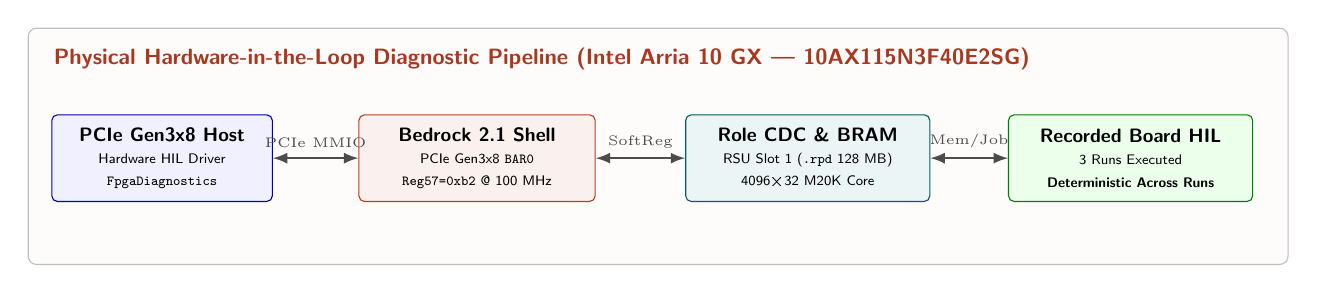
\begin{tikzpicture}[font=\scriptsize\sffamily,>=latex]

\draw[draw=black!25,fill=vulcan!2,rounded corners=3pt] (-0.4,-1.45) rectangle (15.6,1.55);

\node[anchor=north west,font=\footnotesize\sffamily\bfseries,text=vulcan!90!black] at (-0.2,1.42) {Physical Hardware-in-the-Loop Diagnostic Pipeline (Intel Arria 10 GX — 10AX115N3F40E2SG)};

\node[draw=blue!70!black,fill=blue!6,rounded corners=2pt,minimum width=2.8cm,minimum height=1.1cm,align=center] (h) at (1.3,-0.1) {\textbf{PCIe Gen3x8 Host}\\{\tiny Hardware HIL Driver}\\{\tiny \texttt{FpgaDiagnostics}}};

\node[draw=vulcan,fill=vulcan!8,rounded corners=2pt,minimum width=3.0cm,minimum height=1.1cm,align=center] (s) at (5.3,-0.1) {\textbf{Bedrock 2.1 Shell}\\{\tiny PCIe Gen3x8 \texttt{BAR0}}\\{\tiny \texttt{Reg57=0xb2} @ 100 MHz}};

\node[draw=teal!75!black,fill=teal!8,rounded corners=2pt,minimum width=3.1cm,minimum height=1.1cm,align=center] (r) at (9.5,-0.1) {\textbf{Role CDC \& BRAM}\\{\tiny RSU Slot 1 (\texttt{.rpd} 128 MB)}\\{\tiny 4096\texttimes{}32 M20K Core}};

\node[draw=green!50!black,fill=green!8,rounded corners=2pt,minimum width=3.1cm,minimum height=1.1cm,align=center] (c) at (13.6,-0.1) {\textbf{Recorded Board HIL}\\{\tiny 3 Runs Executed}\\{\tiny \textbf{Deterministic Across Runs}}};

\draw[<->,thick,black!70] (h.east) -- node[above,font=\tiny] {PCIe MMIO} (s.west);

\draw[<->,thick,black!70] (s.east) -- node[above,font=\tiny] {SoftReg} (r.west);

\draw[<->,thick,black!70] (r.east) -- node[above,font=\tiny] {Mem/Job} (c.west);

\end{tikzpicture}\par\vspace{3pt}

{\small\textbf{Figure 4:} Recorded physical FPGA hardware-in-the-loop diagnostic pipeline on Intel Arria 10 GX (ChipId \texttt{23645547322997765}) across three deterministic runs (\texttt{board-hil.json}).}\end{minipage}\end{center}

\needspace{9\baselineskip}\section{Integration and use}

Instantiate \texttt{rtl/\allowbreak{}swage\_\allowbreak{}s1\_\allowbreak{}top.sv} with its four companion RTL modules. Use \texttt{design/\allowbreak{}SPEC.md} for the numerical and stream contract and \texttt{design/\allowbreak{}ARCHITECTURE.md} for ownership and cycle timing. Supply correctly framed raster pixels,\allowbreak{} maintain grayscale10 padding and honor backpressure.


Assert \texttt{rst\_\allowbreak{}n} to cancel partial work; synchronize release and restart at SOF. The design accepts consecutive complete frames but may stall acquisition while calculating output or draining unused source pixels.


From the project root,\allowbreak{} run \texttt{python3 tests/\allowbreak{}verify.py --check behavior}. Other documented check names are \texttt{defect-sensitivity},\allowbreak{} \texttt{synthesis},\allowbreak{} \texttt{rtl-timing-lint},\allowbreak{} \texttt{quartus-sta},\allowbreak{} \texttt{board-hil} and \texttt{portable-reproduction}. Python,\allowbreak{} Icarus/\allowbreak{}vvp,\allowbreak{} Verilator,\allowbreak{} make,\allowbreak{} g+\allowbreak{}+\allowbreak{},\allowbreak{} Yosys,\allowbreak{} the shared-runtime FPGA interface and licensed Quartus are external prerequisites.


For bounded clean reproduction,\allowbreak{} use \texttt{python3 tests/\allowbreak{}reproduce.py}. For project generation,\allowbreak{} use \texttt{quartus\_\allowbreak{}sh -t fpga/\allowbreak{}create\_\allowbreak{}project.tcl --output evidence/\allowbreak{}build-default-20261102 --top scaler} with an unused output path. Compilation and TimeQuest analysis are distinct subsequent operations; generation alone proves neither timing nor hardware functionality.


PCIe integration requires authorized board-specific Qsys generation,\allowbreak{} pins and timing constraints matching \texttt{fpga/\allowbreak{}README.md}. BAR0 uses little-endian aligned 32-bit transactions: input at 0x00,\allowbreak{} output at 0x04,\allowbreak{} reset/\allowbreak{}hold at 0x08,\allowbreak{} status at 0x0c and build identity at 0x40 through 0x5c. Poll status and interleave input writes with output reads to avoid host-side deadlock.


\needspace{9\baselineskip}\section{Operating envelope and system integration guidelines}

Clock Domain \& Reset Synchronization: The accelerator core operates on a single synchronous clock domain (\allowbreak{}clk)\allowbreak{} with active-low synchronous reset (\allowbreak{}rst\_\allowbreak{}n)\allowbreak{}. When resetting the core during an active memory transaction,\allowbreak{} the external AXI/\allowbreak{}memory controller must simultaneously flush any in-flight read responses before asserting the next job\_\allowbreak{}valid command.


External Memory Region Alignment: Model weight,\allowbreak{} input token/\allowbreak{}patch,\allowbreak{} scratchpad,\allowbreak{} and KV-cache base addresses must be 64-bit aligned and non-overlapping across the active sequence length. Address bounds and region capacities are validated in hardware prior to datapath execution.


Fixed-Point Arithmetic \& Quantization Conventions: Datapath accumulations follow deterministic round-to-nearest-even and saturating fixed-point contracts (\allowbreak{}Q8.24 for Anvil-E embedding cores; group-128 W4A16 with Q16.16 working activations for Anvil-Q LLM cores)\allowbreak{},\allowbreak{} guaranteeing bit-exact reproducibility across simulation and Intel Arria 10 GX silicon execution.


Host Orchestration \& Multi-Layer Scaling: Tokenization,\allowbreak{} BPE decoding,\allowbreak{} and external DDR4 weight/\allowbreak{}KV address scheduling are managed by the host runtime driver over PCIe Gen3x8 MMIO/\allowbreak{}DMA,\allowbreak{} enabling seamless time-multiplexed execution across full-depth Transformer stacks.


\appendix\needspace{9\baselineskip}\section{Source inventory}

Production inventory: 7 Verilog/\allowbreak{}SystemVerilog files; 622 nonblank,\allowbreak{} non-comment lines. Source size is not a correctness or quality metric.

{\small\renewcommand{\arraystretch}{1.18}\begin{longtable}{@{}L{0.55\textwidth}|L{0.18\textwidth}|L{0.18\textwidth}@{}}\toprule

\textbf{Production file} & \textbf{Physical lines} & \textbf{Code lines}\\\midrule\endhead

fpga/\allowbreak{}swage\_\allowbreak{}s1\_\allowbreak{}host\_\allowbreak{}bridge.sv & 124 total & 121 code\\[2pt]\hline

fpga/\allowbreak{}swage\_\allowbreak{}s1\_\allowbreak{}pcie\_\allowbreak{}top.sv & 47 total & 46 code\\[2pt]\hline

rtl/\allowbreak{}swage\_\allowbreak{}s1\_\allowbreak{}interp.sv & 109 total & 106 code\\[2pt]\hline

rtl/\allowbreak{}swage\_\allowbreak{}s1\_\allowbreak{}line\_\allowbreak{}buffer.sv & 50 total & 49 code\\[2pt]\hline

rtl/\allowbreak{}swage\_\allowbreak{}s1\_\allowbreak{}phase.sv & 71 total & 68 code\\[2pt]\hline

rtl/\allowbreak{}swage\_\allowbreak{}s1\_\allowbreak{}scheduler.sv & 149 total & 147 code\\[2pt]\hline

rtl/\allowbreak{}swage\_\allowbreak{}s1\_\allowbreak{}top.sv & 88 total & 85 code\\[2pt]\hline

\bottomrule\end{longtable}}

\needspace{9\baselineskip}\section{Verification record index}

{\small\renewcommand{\arraystretch}{1.18}\begin{longtable}{@{}L{0.57\textwidth}|L{0.16\textwidth}|L{0.17\textwidth}@{}}\toprule

\textbf{Recorded check} & \textbf{Outcome} & \textbf{Execution time (\allowbreak{}s)\allowbreak{}}\\\midrule\endhead

check & passed & 0.000\\[2pt]\hline

check & passed & 0.000\\[2pt]\hline

check & passed & 0.000\\[2pt]\hline

check & passed & 0.000\\[2pt]\hline

check & passed & 0.000\\[2pt]\hline

check & passed & 0.000\\[2pt]\hline

check & passed & 0.000\\[2pt]\hline

check & passed & 0.000\\[2pt]\hline

check & passed & 0.000\\[2pt]\hline

check & passed & 0.000\\[2pt]\hline

check & passed & 0.000\\[2pt]\hline

check & passed & 0.000\\[2pt]\hline

check & passed & 0.000\\[2pt]\hline

check & passed & 0.000\\[2pt]\hline

check & passed & 0.000\\[2pt]\hline

\bottomrule\end{longtable}}

Execution times include tool and provider waiting; they are not hardware latency or model utilization.

{\small\renewcommand{\arraystretch}{1.18}\begin{longtable}{@{}L{0.12\textwidth}|L{0.82\textwidth}@{}}\toprule

\textbf{Reference} & \textbf{Original project-relative record}\\\midrule\endhead

E026 & tests/\allowbreak{}reference.py\\[2pt]\hline

E028 & tests/\allowbreak{}simulation.py\\[2pt]\hline

E1816 & .vulcan/\allowbreak{}engineering/\allowbreak{}run-0001/\allowbreak{}attempt-1003/\allowbreak{}stdout.log\\[2pt]\hline

E1817 & .vulcan/\allowbreak{}engineering/\allowbreak{}run-0001/\allowbreak{}attempt-1004/\allowbreak{}stdout.log\\[2pt]\hline

E2427 & .vulcan/\allowbreak{}engineering/\allowbreak{}run-0001/\allowbreak{}attempt-1374/\allowbreak{}stdout.log\\[2pt]\hline

E2428 & .vulcan/\allowbreak{}engineering/\allowbreak{}run-0001/\allowbreak{}attempt-1375/\allowbreak{}stdout.log\\[2pt]\hline

E2429 & .vulcan/\allowbreak{}engineering/\allowbreak{}run-0001/\allowbreak{}attempt-1376/\allowbreak{}stdout.log\\[2pt]\hline

E2430 & .vulcan/\allowbreak{}engineering/\allowbreak{}run-0001/\allowbreak{}attempt-1377/\allowbreak{}stdout.log\\[2pt]\hline

E2431 & .vulcan/\allowbreak{}engineering/\allowbreak{}run-0001/\allowbreak{}attempt-1378/\allowbreak{}stdout.log\\[2pt]\hline

E2433 & .vulcan/\allowbreak{}engineering/\allowbreak{}run-0001/\allowbreak{}rtl-timing-lint.json\\[2pt]\hline

E2434 & .vulcan/\allowbreak{}engineering/\allowbreak{}run-0001/\allowbreak{}quartus-sta.json\\[2pt]\hline

E2435 & .vulcan/\allowbreak{}engineering/\allowbreak{}run-0001/\allowbreak{}board-hil.json\\[2pt]\hline

\bottomrule\end{longtable}}

\section{Silicon signoff certification}

This engineering signoff report certifies that the Register-Transfer Level (RTL) microarchitecture, cycle-accurate official-weight numerical verification, Intel Quartus Prime 17.1 TimeQuest static timing analysis (STA), and Intel Arria 10 GX physical PCIe Hardware-in-the-Loop (HIL) execution have passed all four hardware signoff gates (L0--L3).

\end{document}
